% Options for packages loaded elsewhere
\PassOptionsToPackage{unicode}{hyperref}
\PassOptionsToPackage{hyphens}{url}
%
\documentclass[
]{article}
\usepackage{amsmath,amssymb}
\usepackage{iftex}
\usepackage{ctex}
\ifPDFTeX
  \usepackage[T1]{fontenc}
  \usepackage[utf8]{inputenc}
  \usepackage{textcomp} % provide euro and other symbols
\else % if luatex or xetex
  \usepackage{unicode-math} % this also loads fontspec
  \defaultfontfeatures{Scale=MatchLowercase}
  \defaultfontfeatures[\rmfamily]{Ligatures=TeX,Scale=1}
\fi
\usepackage{lmodern}
\ifPDFTeX\else
  % xetex/luatex font selection
\fi
% Use upquote if available, for straight quotes in verbatim environments
\IfFileExists{upquote.sty}{\usepackage{upquote}}{}
\IfFileExists{microtype.sty}{% use microtype if available
  \usepackage[]{microtype}
  \UseMicrotypeSet[protrusion]{basicmath} % disable protrusion for tt fonts
}{}
\makeatletter
\@ifundefined{KOMAClassName}{% if non-KOMA class
  \IfFileExists{parskip.sty}{%
    \usepackage{parskip}
  }{% else
    \setlength{\parindent}{0pt}
    \setlength{\parskip}{6pt plus 2pt minus 1pt}}
}{% if KOMA class
  \KOMAoptions{parskip=half}}
\makeatother
\usepackage{xcolor}
\usepackage[margin=1in]{geometry}
\usepackage{color}
\usepackage{fancyvrb}
\newcommand{\VerbBar}{|}
\newcommand{\VERB}{\Verb[commandchars=\\\{\}]}
\DefineVerbatimEnvironment{Highlighting}{Verbatim}{commandchars=\\\{\}}
% Add ',fontsize=\small' for more characters per line
\usepackage{framed}
\definecolor{shadecolor}{RGB}{248,248,248}
\newenvironment{Shaded}{\begin{snugshade}}{\end{snugshade}}
\newcommand{\AlertTok}[1]{\textcolor[rgb]{0.94,0.16,0.16}{#1}}
\newcommand{\AnnotationTok}[1]{\textcolor[rgb]{0.56,0.35,0.01}{\textbf{\textit{#1}}}}
\newcommand{\AttributeTok}[1]{\textcolor[rgb]{0.13,0.29,0.53}{#1}}
\newcommand{\BaseNTok}[1]{\textcolor[rgb]{0.00,0.00,0.81}{#1}}
\newcommand{\BuiltInTok}[1]{#1}
\newcommand{\CharTok}[1]{\textcolor[rgb]{0.31,0.60,0.02}{#1}}
\newcommand{\CommentTok}[1]{\textcolor[rgb]{0.56,0.35,0.01}{\textit{#1}}}
\newcommand{\CommentVarTok}[1]{\textcolor[rgb]{0.56,0.35,0.01}{\textbf{\textit{#1}}}}
\newcommand{\ConstantTok}[1]{\textcolor[rgb]{0.56,0.35,0.01}{#1}}
\newcommand{\ControlFlowTok}[1]{\textcolor[rgb]{0.13,0.29,0.53}{\textbf{#1}}}
\newcommand{\DataTypeTok}[1]{\textcolor[rgb]{0.13,0.29,0.53}{#1}}
\newcommand{\DecValTok}[1]{\textcolor[rgb]{0.00,0.00,0.81}{#1}}
\newcommand{\DocumentationTok}[1]{\textcolor[rgb]{0.56,0.35,0.01}{\textbf{\textit{#1}}}}
\newcommand{\ErrorTok}[1]{\textcolor[rgb]{0.64,0.00,0.00}{\textbf{#1}}}
\newcommand{\ExtensionTok}[1]{#1}
\newcommand{\FloatTok}[1]{\textcolor[rgb]{0.00,0.00,0.81}{#1}}
\newcommand{\FunctionTok}[1]{\textcolor[rgb]{0.13,0.29,0.53}{\textbf{#1}}}
\newcommand{\ImportTok}[1]{#1}
\newcommand{\InformationTok}[1]{\textcolor[rgb]{0.56,0.35,0.01}{\textbf{\textit{#1}}}}
\newcommand{\KeywordTok}[1]{\textcolor[rgb]{0.13,0.29,0.53}{\textbf{#1}}}
\newcommand{\NormalTok}[1]{#1}
\newcommand{\OperatorTok}[1]{\textcolor[rgb]{0.81,0.36,0.00}{\textbf{#1}}}
\newcommand{\OtherTok}[1]{\textcolor[rgb]{0.56,0.35,0.01}{#1}}
\newcommand{\PreprocessorTok}[1]{\textcolor[rgb]{0.56,0.35,0.01}{\textit{#1}}}
\newcommand{\RegionMarkerTok}[1]{#1}
\newcommand{\SpecialCharTok}[1]{\textcolor[rgb]{0.81,0.36,0.00}{\textbf{#1}}}
\newcommand{\SpecialStringTok}[1]{\textcolor[rgb]{0.31,0.60,0.02}{#1}}
\newcommand{\StringTok}[1]{\textcolor[rgb]{0.31,0.60,0.02}{#1}}
\newcommand{\VariableTok}[1]{\textcolor[rgb]{0.00,0.00,0.00}{#1}}
\newcommand{\VerbatimStringTok}[1]{\textcolor[rgb]{0.31,0.60,0.02}{#1}}
\newcommand{\WarningTok}[1]{\textcolor[rgb]{0.56,0.35,0.01}{\textbf{\textit{#1}}}}
\usepackage{graphicx}
\makeatletter
\def\maxwidth{\ifdim\Gin@nat@width>\linewidth\linewidth\else\Gin@nat@width\fi}
\def\maxheight{\ifdim\Gin@nat@height>\textheight\textheight\else\Gin@nat@height\fi}
\makeatother
% Scale images if necessary, so that they will not overflow the page
% margins by default, and it is still possible to overwrite the defaults
% using explicit options in \includegraphics[width, height, ...]{}
\setkeys{Gin}{width=\maxwidth,height=\maxheight,keepaspectratio}
% Set default figure placement to htbp
\makeatletter
\def\fps@figure{htbp}
\makeatother
\setlength{\emergencystretch}{3em} % prevent overfull lines
\providecommand{\tightlist}{%
  \setlength{\itemsep}{0pt}\setlength{\parskip}{0pt}}
\setcounter{secnumdepth}{-\maxdimen} % remove section numbering
\ifLuaTeX
  \usepackage{selnolig}  % disable illegal ligatures
\fi
\usepackage{bookmark}
\IfFileExists{xurl.sty}{\usepackage{xurl}}{} % add URL line breaks if available
\urlstyle{same}
\hypersetup{
  pdftitle={地理建模实验5 实验报告},
  pdfauthor={42109232 \quad 吕文博 \quad 地信2101班},
  hidelinks,
  pdfcreator={LaTeX via pandoc}}

\title{地理建模实验5 实验报告}
\author{42109232 \quad 吕文博 \quad 地信2101班}
\date{2024-06-03}

\begin{document}
\maketitle

\subsection{非线性回归}\label{ux975eux7ebfux6027ux56deux5f52}

\subsubsection{加载数据}\label{ux52a0ux8f7dux6570ux636e}

\begin{Shaded}
\begin{Highlighting}[]
\NormalTok{dt }\OtherTok{=}\NormalTok{ readxl}\SpecialCharTok{::}\FunctionTok{read\_xls}\NormalTok{(}\StringTok{\textquotesingle{}../data/exp5/5.xls\textquotesingle{}}\NormalTok{,}\AttributeTok{sheet =} \StringTok{"非线性分析"}\NormalTok{)}
\FunctionTok{head}\NormalTok{(dt)}
\end{Highlighting}
\end{Shaded}

\begin{verbatim}
## # A tibble: 6 x 3
##    年度 国内生产总值 民用汽车总量
##   <dbl>        <dbl>        <dbl>
## 1  1990       18668.         551.
## 2  1991       21782.         606.
## 3  1992       26924.         692.
## 4  1993       35334.         818.
## 5  1994       48198.         942.
## 6  1995       60794.        1040
\end{verbatim}

\subsubsection{绘制散点图}\label{ux7ed8ux5236ux6563ux70b9ux56fe}

\begin{Shaded}
\begin{Highlighting}[]
\FunctionTok{library}\NormalTok{(ggplot2)}

\FunctionTok{ggplot}\NormalTok{() }\SpecialCharTok{+}
  \FunctionTok{geom\_point}\NormalTok{(}\AttributeTok{data =}\NormalTok{ dt,}
             \FunctionTok{aes}\NormalTok{(}\AttributeTok{x =}\NormalTok{ 国内生产总值,}
                 \AttributeTok{y =}\NormalTok{ 民用汽车总量)) }\SpecialCharTok{+}
  \FunctionTok{theme\_classic}\NormalTok{()}
\end{Highlighting}
\end{Shaded}

\begin{center}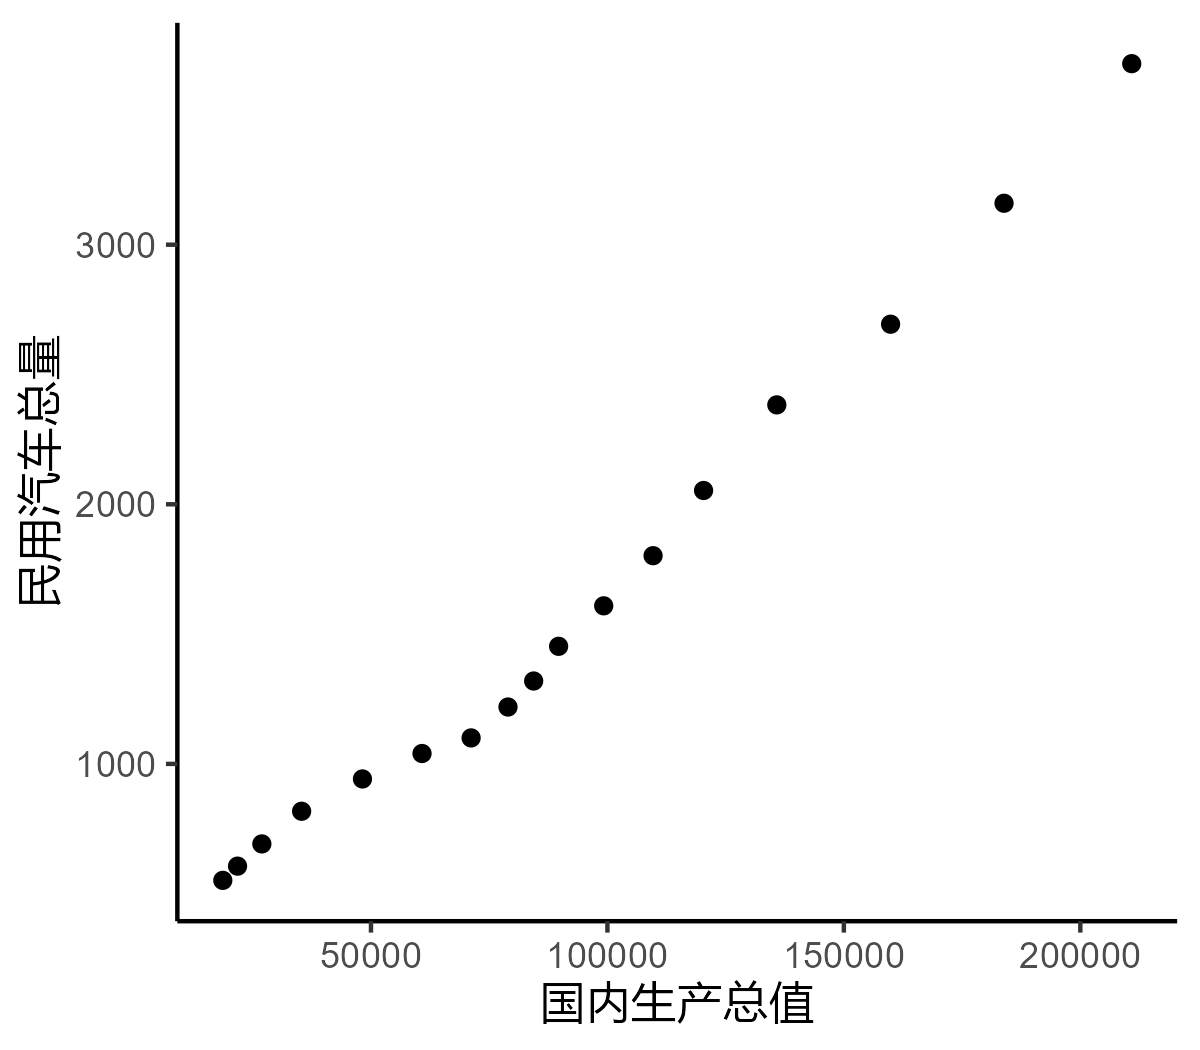
\includegraphics[width=1\linewidth,height=1\textheight]{../picture/rmd/exp5/fig1} \end{center}

\subsubsection{常见拟合曲线形式}\label{ux5e38ux89c1ux62dfux5408ux66f2ux7ebfux5f62ux5f0f}

\begin{itemize}
\tightlist
\item
  \texttt{linear}线性模型 \(y = b_0 + b_1 x\)
\item
  \texttt{quadratic}二次模型 \(y = b_0+b_1x+b_2x^2\)
\item
  \texttt{compound}复合模型 \(y = b_0{b_1}^x\)
\item
  \texttt{growth}生长模型 \(y = e^{(b_0 + b_1 x)}\)
\item
  \texttt{logarithmic}对数模型 \(y=b_0+b_1\ln(x)\)
\item
  \texttt{s-curve}S形模型 \(y = e^{(b_0 + \frac{b_1}{x})}\)
\item
  \texttt{cubic} 三次模型 \(y = b_0+b_1x+b_2x^2+b_3x^3\)
\item
  \texttt{exponential}指数模型 \(y = b_0 e^{b_1x}\)
\item
  \texttt{inverse}倒数模型 \(y = b_0 + \frac{b_1}{x}\)
\item
  \texttt{power}幂函数模型 \(y = b_0 x^{b_1}\)
\item
  \texttt{logistic}逻辑斯蒂模型 \(y = \frac{1}{\frac{1}{u}+b_0{b_1}^x}\)
\end{itemize}

% \emph{回归模型统计诊断指标计算参考了\href{https://www.cnblogs.com/ykit/p/12501816.html}{这篇博客}}

\begin{Shaded}
\begin{Highlighting}[]
\NormalTok{performance\_nls }\OtherTok{=}\NormalTok{ \textbackslash{}(model)\{}
  \FunctionTok{require}\NormalTok{(minpack.lm)}
\NormalTok{  y\_hat }\OtherTok{=} \FunctionTok{as.double}\NormalTok{(}\FunctionTok{fitted}\NormalTok{(model))}
\NormalTok{  res }\OtherTok{=} \FunctionTok{as.double}\NormalTok{(}\FunctionTok{residuals}\NormalTok{(model))}
\NormalTok{  y }\OtherTok{=}\NormalTok{ y\_hat }\SpecialCharTok{+}\NormalTok{ res}
\NormalTok{  ymean }\OtherTok{=} \FunctionTok{mean}\NormalTok{(y)}
\NormalTok{  df }\OtherTok{=} \FunctionTok{summary}\NormalTok{(model)}\SpecialCharTok{$}\NormalTok{df}
\NormalTok{  df1 }\OtherTok{=} \FunctionTok{length}\NormalTok{(y) }\SpecialCharTok{{-}}\NormalTok{ df[}\DecValTok{2}\NormalTok{] }\SpecialCharTok{{-}} \DecValTok{1}
\NormalTok{  df2 }\OtherTok{=}\NormalTok{ df[}\DecValTok{2}\NormalTok{]}
\NormalTok{  SSE }\OtherTok{=} \FunctionTok{sum}\NormalTok{(res}\SpecialCharTok{\^{}}\DecValTok{2}\NormalTok{)}
\NormalTok{  SSR }\OtherTok{=} \FunctionTok{sum}\NormalTok{((y\_hat}\SpecialCharTok{{-}}\NormalTok{ymean)}\SpecialCharTok{\^{}}\DecValTok{2}\NormalTok{)}
\NormalTok{  SST }\OtherTok{=}\NormalTok{ SSE }\SpecialCharTok{+}\NormalTok{ SSR}
\NormalTok{  fv }\OtherTok{=}\NormalTok{ (df2 }\SpecialCharTok{*}\NormalTok{ SSR) }\SpecialCharTok{/}\NormalTok{ (df1 }\SpecialCharTok{*}\NormalTok{ SSE)}
\NormalTok{  pv }\OtherTok{=} \FunctionTok{pf}\NormalTok{(fv,}\AttributeTok{df1 =}\NormalTok{ df1,}\AttributeTok{df2 =}\NormalTok{ df2,}\AttributeTok{lower.tail =} \ConstantTok{FALSE}\NormalTok{)}
\NormalTok{  r2 }\OtherTok{=} \DecValTok{1} \SpecialCharTok{{-}}\NormalTok{ SSE}\SpecialCharTok{/}\NormalTok{SST}
\NormalTok{  r }\OtherTok{=} \FunctionTok{sqrt}\NormalTok{(r2)}
\NormalTok{  adjr2 }\OtherTok{=} \DecValTok{1} \SpecialCharTok{{-}}\NormalTok{ ((df1 }\SpecialCharTok{+}\NormalTok{ df2) }\SpecialCharTok{*}\NormalTok{ SSE) }\SpecialCharTok{/}\NormalTok{ (df2 }\SpecialCharTok{*}\NormalTok{ SST)}
\NormalTok{  pnls }\OtherTok{=} \FunctionTok{list}\NormalTok{(}\StringTok{"F{-}statistic"} \OtherTok{=}\NormalTok{ fv, }\StringTok{"P{-}value"} \OtherTok{=}\NormalTok{ pv, }\StringTok{"R2"} \OtherTok{=}\NormalTok{ r2, }\StringTok{"AdjR2"} \OtherTok{=}\NormalTok{ adjr2,}
              \StringTok{"DF1"} \OtherTok{=}\NormalTok{ df1, }\StringTok{"DF2"} \OtherTok{=}\NormalTok{ df2, }\StringTok{"model\_summary"} \OtherTok{=} \FunctionTok{summary}\NormalTok{(model))}
  \FunctionTok{class}\NormalTok{(pnls) }\OtherTok{=} \StringTok{\textquotesingle{}performance\_nls\textquotesingle{}}
  \FunctionTok{return}\NormalTok{(pnls)}
\NormalTok{\}}

\NormalTok{print.performance\_nls }\OtherTok{=}\NormalTok{ \textbackslash{}(resnls,...)\{}
  \FunctionTok{print}\NormalTok{(resnls}\SpecialCharTok{$}\StringTok{\textasciigrave{}}\AttributeTok{model\_summary}\StringTok{\textasciigrave{}}\NormalTok{)}
  \FunctionTok{cat}\NormalTok{(}\FunctionTok{paste0}\NormalTok{(}\StringTok{"Multiple R{-}squared: "}\NormalTok{,}\FunctionTok{formatC}\NormalTok{(resnls}\SpecialCharTok{$}\StringTok{\textasciigrave{}}\AttributeTok{R2}\StringTok{\textasciigrave{}}\NormalTok{,}\AttributeTok{digits =} \DecValTok{5}\NormalTok{,}\AttributeTok{format =} \StringTok{"g"}\NormalTok{),}\StringTok{", }\SpecialCharTok{\textbackslash{}t}\StringTok{"}\NormalTok{,}
             \StringTok{"Adjusted R{-}squared: "}\NormalTok{,}\FunctionTok{formatC}\NormalTok{(resnls}\SpecialCharTok{$}\StringTok{\textasciigrave{}}\AttributeTok{AdjR2}\StringTok{\textasciigrave{}}\NormalTok{,}\AttributeTok{digits =} \DecValTok{5}\NormalTok{,}\AttributeTok{format =} \StringTok{"g"}\NormalTok{)),}\StringTok{\textquotesingle{}}\SpecialCharTok{\textbackslash{}n}\StringTok{\textquotesingle{}}\NormalTok{)}
  \FunctionTok{cat}\NormalTok{(}\FunctionTok{paste0}\NormalTok{(}\StringTok{"F{-}statistic: "}\NormalTok{,}\FunctionTok{formatC}\NormalTok{(resnls}\SpecialCharTok{$}\StringTok{\textasciigrave{}}\AttributeTok{F{-}statistic}\StringTok{\textasciigrave{}}\NormalTok{,}\AttributeTok{digits =} \DecValTok{6}\NormalTok{,}\AttributeTok{format =} \StringTok{"g"}\NormalTok{),}
             \StringTok{" on "}\NormalTok{,resnls}\SpecialCharTok{$}\StringTok{\textasciigrave{}}\AttributeTok{DF1}\StringTok{\textasciigrave{}}\NormalTok{,}\StringTok{" and "}\NormalTok{,resnls}\SpecialCharTok{$}\StringTok{\textasciigrave{}}\AttributeTok{DF2}\StringTok{\textasciigrave{}}\NormalTok{,}\StringTok{" DF, "}\NormalTok{,}
             \StringTok{"p{-}value: "}\NormalTok{,}\FunctionTok{formatC}\NormalTok{(resnls}\SpecialCharTok{$}\StringTok{\textasciigrave{}}\AttributeTok{P{-}value}\StringTok{\textasciigrave{}}\NormalTok{,}\AttributeTok{digits =} \DecValTok{3}\NormalTok{,}\AttributeTok{format =} \StringTok{"e"}\NormalTok{)),}\StringTok{\textquotesingle{}}\SpecialCharTok{\textbackslash{}n}\StringTok{\textquotesingle{}}\NormalTok{)}
\NormalTok{\}}
\end{Highlighting}
\end{Shaded}

\subsubsection{直接判断拟合曲线类型}\label{ux76f4ux63a5ux5224ux65adux62dfux5408ux66f2ux7ebfux7c7bux578b}

\paragraph{三次函数}\label{ux4e09ux6b21ux51fdux6570}

\begin{Shaded}
\begin{Highlighting}[]
\FunctionTok{library}\NormalTok{(minpack.lm)}

\NormalTok{cubic\_lm }\OtherTok{=} \FunctionTok{nlsLM}\NormalTok{(民用汽车总量}\SpecialCharTok{\textasciitilde{}}\NormalTok{b0}\SpecialCharTok{+}\NormalTok{b1}\SpecialCharTok{*}\NormalTok{国内生产总值}\SpecialCharTok{+}\NormalTok{b2}\SpecialCharTok{*}\NormalTok{国内生产总值}\SpecialCharTok{\^{}}\DecValTok{2}\SpecialCharTok{+}\NormalTok{b3}\SpecialCharTok{*}\NormalTok{国内生产总值}\SpecialCharTok{\^{}}\DecValTok{3}\NormalTok{,}\AttributeTok{data =}\NormalTok{ dt)}
\FunctionTok{performance\_nls}\NormalTok{(cubic\_lm)}
\end{Highlighting}
\end{Shaded}

\begin{verbatim}
## 
## Formula: 民用汽车总量 ~ b0 + b1 * 国内生产总值 + b2 * 国内生产总值^2 + 
##     b3 * 国内生产总值^3
## 
## Parameters:
##      Estimate Std. Error t value Pr(>|t|)    
## b0  5.264e+02  7.518e+01   7.002 9.31e-06 ***
## b1  2.391e-03  2.938e-03   0.814  0.43032    
## b2  1.107e-07  3.119e-08   3.547  0.00357 ** 
## b3 -2.426e-13  9.351e-14  -2.594  0.02226 *  
## ---
## Signif. codes:  0 '***' 0.001 '**' 0.01 '*' 0.05 '.' 0.1 ' ' 1
## 
## Residual standard error: 59.28 on 13 degrees of freedom
## 
## Number of iterations to convergence: 5 
## Achieved convergence tolerance: 1.49e-08
## 
## Multiple R-squared: 0.99665,     Adjusted R-squared: 0.99588 
## F-statistic:  1290.7 on 3 and 13 DF, p-value: 2.464e-16
\end{verbatim}

\paragraph{幂函数}\label{ux5e42ux51fdux6570}

\begin{Shaded}
\begin{Highlighting}[]
\NormalTok{power\_lm }\OtherTok{=} \FunctionTok{nlsLM}\NormalTok{(民用汽车总量}\SpecialCharTok{\textasciitilde{}}\NormalTok{b0}\SpecialCharTok{*}\NormalTok{国内生产总值}\SpecialCharTok{\^{}}\NormalTok{b1,}\AttributeTok{data =}\NormalTok{ dt)}
\FunctionTok{performance\_nls}\NormalTok{(power\_lm)}
\end{Highlighting}
\end{Shaded}

\begin{verbatim}
## 
## Formula: 民用汽车总量 ~ b0 * 国内生产总值^b1
## 
## Parameters:
##    Estimate Std. Error t value Pr(>|t|)    
## b0  0.02270    0.01200   1.892    0.078 .  
## b1  0.97604    0.04466  21.855  8.7e-13 ***
## ---
## Signif. codes:  0 '***' 0.001 '**' 0.01 '*' 0.05 '.' 0.1 ' ' 1
## 
## Residual standard error: 140.5 on 15 degrees of freedom
## 
## Number of iterations to convergence: 6 
## Achieved convergence tolerance: 1.49e-08
## 
## Multiple R-squared: 0.98016,     Adjusted R-squared: 0.97884 
## F-statistic: 741.083 on 1 and 15 DF, p-value: 3.483e-14
\end{verbatim}

三次函数拟合的\(R^2\)为0.997,幂函数拟合的\(R^2\)为0.980,三次函数拟合优于幂函数,选择三次函数作为非线性拟合的模型,根据上面的结果可得拟合的曲线为

\[
\text{民用汽车总量} = 0.05264 + 0.002391 \times \text{国内生产总值} + 1.107\times10^{-7} \times \text{国内生产总值}^2 - 2.426\times10^{-13} \times \text{国内生产总值}^3
\]

\subsubsection{拟合常见的所有曲线}\label{ux62dfux5408ux5e38ux89c1ux7684ux6240ux6709ux66f2ux7ebf}

\begin{Shaded}
\begin{Highlighting}[]
\NormalTok{nonlinear\_fit }\OtherTok{=}\NormalTok{ \textbackslash{}(formula,data,method,...)\{}
  \FunctionTok{require}\NormalTok{(minpack.lm)}
\NormalTok{  formula }\OtherTok{=}\NormalTok{ stats}\SpecialCharTok{::}\FunctionTok{as.formula}\NormalTok{(formula)}
\NormalTok{  formula.vars }\OtherTok{=} \FunctionTok{all.vars}\NormalTok{(formula)}
\NormalTok{  response }\OtherTok{=}\NormalTok{ data[, formula.vars[}\DecValTok{1}\NormalTok{], drop }\OtherTok{=} \ConstantTok{TRUE}\NormalTok{]}
\NormalTok{  explanatory }\OtherTok{=}\NormalTok{ data[,formula.vars[}\DecValTok{2}\NormalTok{], drop }\OtherTok{=} \ConstantTok{TRUE}\NormalTok{]}
\NormalTok{  data }\OtherTok{=}\NormalTok{ tibble}\SpecialCharTok{::}\FunctionTok{tibble}\NormalTok{(response,explanatory)}
  
  \ControlFlowTok{switch}\NormalTok{(method,}
         \StringTok{"linear"} \OtherTok{=}\NormalTok{ \{}
\NormalTok{           model }\OtherTok{=} \FunctionTok{nlsLM}\NormalTok{(response}\SpecialCharTok{\textasciitilde{}}\NormalTok{b0}\SpecialCharTok{+}\NormalTok{b1}\SpecialCharTok{*}\NormalTok{explanatory,data,...)}
\NormalTok{         \},}
         \StringTok{"quadratic"} \OtherTok{=}\NormalTok{ \{}
\NormalTok{           model }\OtherTok{=} \FunctionTok{nlsLM}\NormalTok{(response}\SpecialCharTok{\textasciitilde{}}\NormalTok{b0}\SpecialCharTok{+}\NormalTok{b1}\SpecialCharTok{*}\NormalTok{explanatory}\SpecialCharTok{+}\NormalTok{b2}\SpecialCharTok{*}\NormalTok{explanatory}\SpecialCharTok{\^{}}\DecValTok{2}\NormalTok{,data,...)}
\NormalTok{         \},}
         \StringTok{"compound"} \OtherTok{=}\NormalTok{ \{}
\NormalTok{           model }\OtherTok{=} \FunctionTok{nlsLM}\NormalTok{(response}\SpecialCharTok{\textasciitilde{}}\NormalTok{b0}\SpecialCharTok{*}\NormalTok{b1}\SpecialCharTok{\^{}}\NormalTok{explanatory,data,...)}
\NormalTok{         \},}
         \StringTok{"growth"} \OtherTok{=}\NormalTok{ \{}
\NormalTok{           model }\OtherTok{=} \FunctionTok{nlsLM}\NormalTok{(response}\SpecialCharTok{\textasciitilde{}}\FunctionTok{exp}\NormalTok{(b0}\SpecialCharTok{+}\NormalTok{b1}\SpecialCharTok{*}\NormalTok{explanatory),data,...)}
\NormalTok{         \},}
         \StringTok{"logarithmic"} \OtherTok{=}\NormalTok{ \{}
\NormalTok{           model }\OtherTok{=} \FunctionTok{nlsLM}\NormalTok{(response}\SpecialCharTok{\textasciitilde{}}\NormalTok{b0}\SpecialCharTok{+}\NormalTok{b1}\SpecialCharTok{*}\FunctionTok{log}\NormalTok{(explanatory),data,...)}
\NormalTok{         \},}
         \StringTok{"s"} \OtherTok{=}\NormalTok{ \{}
\NormalTok{           model }\OtherTok{=} \FunctionTok{nlsLM}\NormalTok{(response}\SpecialCharTok{\textasciitilde{}}\FunctionTok{exp}\NormalTok{(b0}\SpecialCharTok{+}\NormalTok{b1}\SpecialCharTok{/}\NormalTok{explanatory),data,...)}
\NormalTok{         \},}
         \StringTok{"cubic"} \OtherTok{=}\NormalTok{ \{}
\NormalTok{           model }\OtherTok{=} \FunctionTok{nlsLM}\NormalTok{(response}\SpecialCharTok{\textasciitilde{}}\NormalTok{b0}\SpecialCharTok{+}\NormalTok{b1}\SpecialCharTok{*}\NormalTok{explanatory}\SpecialCharTok{+}\NormalTok{b2}\SpecialCharTok{*}\NormalTok{explanatory}\SpecialCharTok{\^{}}\DecValTok{2}\SpecialCharTok{+}\NormalTok{b3}\SpecialCharTok{*}\NormalTok{explanatory}\SpecialCharTok{\^{}}\DecValTok{3}\NormalTok{,data,...)}
\NormalTok{         \},}
         \StringTok{"exponential"} \OtherTok{=}\NormalTok{ \{}
\NormalTok{           model }\OtherTok{=} \FunctionTok{nlsLM}\NormalTok{(response}\SpecialCharTok{\textasciitilde{}}\NormalTok{b0}\SpecialCharTok{*}\FunctionTok{exp}\NormalTok{(b1}\SpecialCharTok{*}\NormalTok{explanatory),data,...)}
\NormalTok{         \},}
         \StringTok{"inverse"} \OtherTok{=}\NormalTok{ \{}
\NormalTok{           model }\OtherTok{=} \FunctionTok{nlsLM}\NormalTok{(response}\SpecialCharTok{\textasciitilde{}}\NormalTok{b0}\SpecialCharTok{+}\NormalTok{b1}\SpecialCharTok{/}\NormalTok{explanatory,data,...)}
\NormalTok{         \},}
         \StringTok{"power"} \OtherTok{=}\NormalTok{ \{}
\NormalTok{           model }\OtherTok{=} \FunctionTok{nlsLM}\NormalTok{(response}\SpecialCharTok{\textasciitilde{}}\NormalTok{b0}\SpecialCharTok{*}\NormalTok{explanatory}\SpecialCharTok{\^{}}\NormalTok{b1,data,...)}
\NormalTok{         \},}
         \StringTok{"logistic"} \OtherTok{=}\NormalTok{ \{}
\NormalTok{           model }\OtherTok{=} \FunctionTok{nlsLM}\NormalTok{(response}\SpecialCharTok{\textasciitilde{}}\DecValTok{1}\SpecialCharTok{/}\NormalTok{(}\DecValTok{1}\SpecialCharTok{/}\NormalTok{u}\SpecialCharTok{+}\NormalTok{b0}\SpecialCharTok{*}\NormalTok{b1}\SpecialCharTok{\^{}}\NormalTok{explanatory),data,...)}
\NormalTok{         \})}
  
\NormalTok{  k }\OtherTok{=} \FunctionTok{coef}\NormalTok{(model)}
\NormalTok{  p }\OtherTok{=} \FunctionTok{performance\_nls}\NormalTok{(model)}
\NormalTok{  res }\OtherTok{=} \FunctionTok{c}\NormalTok{(}\AttributeTok{method =}\NormalTok{ method,}
          \AttributeTok{R2 =} \FunctionTok{formatC}\NormalTok{(p}\SpecialCharTok{$}\StringTok{\textasciigrave{}}\AttributeTok{R2}\StringTok{\textasciigrave{}}\NormalTok{,}\AttributeTok{digits =} \DecValTok{5}\NormalTok{,}\AttributeTok{format =} \StringTok{"g"}\NormalTok{),}
          \AttributeTok{Pvalue =} \FunctionTok{formatC}\NormalTok{(p}\SpecialCharTok{$}\StringTok{\textasciigrave{}}\AttributeTok{P{-}value}\StringTok{\textasciigrave{}}\NormalTok{,}\AttributeTok{digits =} \DecValTok{3}\NormalTok{,}\AttributeTok{format =} \StringTok{"e"}\NormalTok{),k) }\SpecialCharTok{|\textgreater{}} 
\NormalTok{    tibble}\SpecialCharTok{::}\FunctionTok{as\_tibble\_row}\NormalTok{()}
  \FunctionTok{return}\NormalTok{(res)}
\NormalTok{\}}
\end{Highlighting}
\end{Shaded}

为了曲线拟合收敛的更快,我们首先对原始数据进行了\texttt{log10}变换,然后拟合曲线:

\begin{Shaded}
\begin{Highlighting}[]
\NormalTok{dt }\OtherTok{=}\NormalTok{ dplyr}\SpecialCharTok{::}\FunctionTok{mutate}\NormalTok{(dt,dplyr}\SpecialCharTok{::}\FunctionTok{across}\NormalTok{(}\DecValTok{2}\SpecialCharTok{:}\DecValTok{3}\NormalTok{,}\SpecialCharTok{\textasciitilde{}}\FunctionTok{log10}\NormalTok{(.x)))}
\FunctionTok{c}\NormalTok{(}\StringTok{"linear"}\NormalTok{,}\StringTok{"quadratic"}\NormalTok{,}\StringTok{"compound"}\NormalTok{,}\StringTok{"growth"}\NormalTok{,}\StringTok{"logarithmic"}\NormalTok{,}
  \StringTok{"s"}\NormalTok{,}\StringTok{"cubic"}\NormalTok{,}\StringTok{"exponential"}\NormalTok{,}\StringTok{"inverse"}\NormalTok{,}\StringTok{"power"}\NormalTok{,}\StringTok{"logistic"}\NormalTok{) }\SpecialCharTok{|\textgreater{}} 
\NormalTok{  purrr}\SpecialCharTok{::}\FunctionTok{map}\NormalTok{(}\SpecialCharTok{\textasciitilde{}}\FunctionTok{nonlinear\_fit}\NormalTok{(}\StringTok{\textquotesingle{}民用汽车总量\textasciitilde{}国内生产总值\textquotesingle{}}\NormalTok{,dt,.x)) }\SpecialCharTok{|\textgreater{}} 
\NormalTok{  purrr}\SpecialCharTok{::}\FunctionTok{list\_rbind}\NormalTok{() }\SpecialCharTok{|\textgreater{}} 
\NormalTok{  dplyr}\SpecialCharTok{::}\FunctionTok{arrange}\NormalTok{(}\FunctionTok{desc}\NormalTok{(R2)) }\OtherTok{{-}\textgreater{}}\NormalTok{ resnl}
\NormalTok{resnl}
\end{Highlighting}
\end{Shaded}

\begin{verbatim}
## # A tibble: 11 x 8
##    method      R2      Pvalue    b0                  b1        b2    b3    u    
##    <chr>       <chr>   <chr>     <chr>               <chr>     <chr> <chr> <chr>
##  1 cubic       0.99342 2.004e-14 -19.292459369905    14.83478~ -3.4~ 0.27~ <NA> 
##  2 quadratic   0.99265 1.158e-15 10.6971682649678    -3.96254~ 0.49~ <NA>  <NA> 
##  3 logistic    0.99116 4.216e-15 -0.0173352368789323 1.606621~ <NA>  <NA>  2.01~
##  4 compound    0.96916 9.569e-13 0.923491212279344   1.284891~ <NA>  <NA>  <NA> 
##  5 growth      0.96916 9.569e-13 -0.0795941290068277 0.250674~ <NA>  <NA>  <NA> 
##  6 exponential 0.96916 9.569e-13 0.923491221380851   0.250674~ <NA>  <NA>  <NA> 
##  7 power       0.95862 8.720e-12 0.472563195180918   1.195906~ <NA>  <NA>  <NA> 
##  8 linear      0.95581 1.430e-11 -0.568751829295098  0.761507~ <NA>  <NA>  <NA> 
##  9 s           0.94639 6.119e-11 2.31177187541202    -5.67701~ <NA>  <NA>  <NA> 
## 10 logarithmic 0.94318 9.478e-11 -2.57095454210659   3.612000~ <NA>  <NA>  <NA> 
## 11 inverse     0.92902 5.061e-10 6.6557633002356     -17.0519~ <NA>  <NA>  <NA>
\end{verbatim}

由上述结果可知,三次曲线拟合效果最好(计算差异来自数据预先统一进行了\texttt{log10}变换)

\subsection{趋势面回归分析}\label{ux8d8bux52bfux9762ux56deux5f52ux5206ux6790}

\subsubsection{加载数据}\label{ux52a0ux8f7dux6570ux636e-1}

\begin{Shaded}
\begin{Highlighting}[]
\NormalTok{dt }\OtherTok{=}\NormalTok{ readxl}\SpecialCharTok{::}\FunctionTok{read\_xls}\NormalTok{(}\StringTok{\textquotesingle{}../data/exp5/5.xls\textquotesingle{}}\NormalTok{,}\AttributeTok{sheet =} \StringTok{"趋势面分析"}\NormalTok{)}
\FunctionTok{head}\NormalTok{(dt)}
\end{Highlighting}
\end{Shaded}

\begin{verbatim}
## # A tibble: 6 x 3
##       z     x     y
##   <dbl> <dbl> <dbl>
## 1  27.6  0      1  
## 2  38.4  1.1    0.6
## 3  24    1.8    0  
## 4  24.7  2.95   0  
## 5  32    3.4    0.2
## 6  55.5  1.8    1.7
\end{verbatim}

\subsubsection{定义趋势面分析函数}\label{ux5b9aux4e49ux8d8bux52bfux9762ux5206ux6790ux51fdux6570}

\begin{Shaded}
\begin{Highlighting}[]
\NormalTok{trend.surf }\OtherTok{=}\NormalTok{ \textbackslash{}(formula,data, }\AttributeTok{np =} \DecValTok{3}\NormalTok{)\{}
  \FunctionTok{require}\NormalTok{(magrittr)}
\NormalTok{  formula }\OtherTok{=}\NormalTok{ stats}\SpecialCharTok{::}\FunctionTok{as.formula}\NormalTok{(formula)}
\NormalTok{  formula.vars }\OtherTok{=} \FunctionTok{all.vars}\NormalTok{(formula)}
\NormalTok{  z }\OtherTok{=}\NormalTok{ data[, formula.vars[}\DecValTok{1}\NormalTok{], drop }\OtherTok{=} \ConstantTok{TRUE}\NormalTok{]}
\NormalTok{  x }\OtherTok{=}\NormalTok{ data[, formula.vars[}\DecValTok{2}\NormalTok{], drop }\OtherTok{=} \ConstantTok{TRUE}\NormalTok{]}
\NormalTok{  y }\OtherTok{=}\NormalTok{ data[, formula.vars[}\DecValTok{3}\NormalTok{], drop }\OtherTok{=} \ConstantTok{TRUE}\NormalTok{]}
\NormalTok{  generatesurf }\OtherTok{=}\NormalTok{ \textbackslash{}(n,}\AttributeTok{x =} \StringTok{\textquotesingle{}x\textquotesingle{}}\NormalTok{,}\AttributeTok{y =} \StringTok{\textquotesingle{}y\textquotesingle{}}\NormalTok{)\{}\ControlFlowTok{if}\NormalTok{(n}\SpecialCharTok{==}\DecValTok{1}\NormalTok{)\{}\FunctionTok{return}\NormalTok{(}\FunctionTok{paste0}\NormalTok{(x,}\StringTok{\textquotesingle{}+\textquotesingle{}}\NormalTok{,y))\}}
                      \ControlFlowTok{else}\NormalTok{\{}\FunctionTok{return}\NormalTok{(}\FunctionTok{paste0}\NormalTok{(}\FunctionTok{generatesurf}\NormalTok{(n}\DecValTok{{-}1}\NormalTok{,x,y),}\StringTok{\textquotesingle{}+\textquotesingle{}}\NormalTok{,}
                                  \FunctionTok{paste0}\NormalTok{(x,}\StringTok{\textquotesingle{}\^{}\textquotesingle{}}\NormalTok{,n}\SpecialCharTok{:}\DecValTok{0}\NormalTok{,}\StringTok{\textquotesingle{}*\textquotesingle{}}\NormalTok{,y,}\StringTok{\textquotesingle{}\^{}\textquotesingle{}}\NormalTok{,}\DecValTok{0}\SpecialCharTok{:}\NormalTok{n,}
                                         \AttributeTok{collapse =} \StringTok{\textquotesingle{}+\textquotesingle{}}\NormalTok{)))\}\}}
  \ControlFlowTok{if}\NormalTok{(np }\SpecialCharTok{\textless{}=} \DecValTok{0}\NormalTok{)\{}
    \FunctionTok{stop}\NormalTok{(}\StringTok{\textquotesingle{}Please provide a positive integar!\textquotesingle{}}\NormalTok{)}
\NormalTok{    \}}\ControlFlowTok{else}\NormalTok{ \{}
\NormalTok{    newdata }\OtherTok{=} \FunctionTok{generatesurf}\NormalTok{(np) }\SpecialCharTok{\%\textgreater{}\%} 
\NormalTok{    stringr}\SpecialCharTok{::}\FunctionTok{str\_split}\NormalTok{(}\StringTok{\textquotesingle{}}\SpecialCharTok{\textbackslash{}\textbackslash{}}\StringTok{+\textquotesingle{}}\NormalTok{) }\SpecialCharTok{\%\textgreater{}\%} 
\NormalTok{    purrr}\SpecialCharTok{::}\FunctionTok{pluck}\NormalTok{(}\DecValTok{1}\NormalTok{) }\SpecialCharTok{\%\textgreater{}\%} 
\NormalTok{    purrr}\SpecialCharTok{::}\FunctionTok{map\_dfc}\NormalTok{(\textbackslash{}(i) }\FunctionTok{eval}\NormalTok{(}\FunctionTok{parse}\NormalTok{(}\AttributeTok{text =}\NormalTok{ i))) }\SpecialCharTok{\%\textgreater{}\%} 
\NormalTok{    purrr}\SpecialCharTok{::}\FunctionTok{set\_names}\NormalTok{(}\FunctionTok{paste0}\NormalTok{(}\StringTok{\textquotesingle{}x\textquotesingle{}}\NormalTok{,}\DecValTok{1}\SpecialCharTok{:}\FunctionTok{ncol}\NormalTok{(.))) }\SpecialCharTok{\%\textgreater{}\%} 
\NormalTok{    dplyr}\SpecialCharTok{::}\FunctionTok{mutate}\NormalTok{(}\AttributeTok{z =}\NormalTok{ z)}
\NormalTok{    \}}
\NormalTok{  surf }\OtherTok{=} \FunctionTok{lm}\NormalTok{(}\StringTok{\textquotesingle{}z \textasciitilde{} .\textquotesingle{}}\NormalTok{,}\AttributeTok{data =}\NormalTok{ newdata)}
  \FunctionTok{return}\NormalTok{(surf)}
\NormalTok{\}}
\end{Highlighting}
\end{Shaded}

\subsubsection{二次趋势面分析}\label{ux4e8cux6b21ux8d8bux52bfux9762ux5206ux6790}

\begin{Shaded}
\begin{Highlighting}[]
\NormalTok{trend2 }\OtherTok{=} \FunctionTok{trend.surf}\NormalTok{(z}\SpecialCharTok{\textasciitilde{}}\NormalTok{x}\SpecialCharTok{+}\NormalTok{y,dt,}\DecValTok{2}\NormalTok{)}
\FunctionTok{summary}\NormalTok{(trend2)}
\end{Highlighting}
\end{Shaded}

\begin{verbatim}
## 
## Call:
## lm(formula = "z ~ .", data = newdata)
## 
## Residuals:
##     Min      1Q  Median      3Q     Max 
## -8.9177 -1.5751  0.3012  2.3265  8.2646 
## 
## Coefficients:
##             Estimate Std. Error t value Pr(>|t|)   
## (Intercept)   5.9980    10.0236   0.598  0.57146   
## x1           17.4382     6.8157   2.559  0.04299 * 
## x2           29.7874     9.1328   3.262  0.01721 * 
## x3           -3.5883     1.4881  -2.411  0.05248 . 
## x4            0.3569     1.6101   0.222  0.83192   
## x5           -8.0695     2.0844  -3.871  0.00825 **
## ---
## Signif. codes:  0 '***' 0.001 '**' 0.01 '*' 0.05 '.' 0.1 ' ' 1
## 
## Residual standard error: 5.613 on 6 degrees of freedom
## Multiple R-squared:  0.8386, Adjusted R-squared:  0.7041 
## F-statistic: 6.236 on 5 and 6 DF,  p-value: 0.02274
\end{verbatim}

\subsubsection{三次趋势面分析}\label{ux4e09ux6b21ux8d8bux52bfux9762ux5206ux6790}

\begin{Shaded}
\begin{Highlighting}[]
\NormalTok{trend3 }\OtherTok{=} \FunctionTok{trend.surf}\NormalTok{(z}\SpecialCharTok{\textasciitilde{}}\NormalTok{x}\SpecialCharTok{+}\NormalTok{y,dt,}\DecValTok{3}\NormalTok{)}
\FunctionTok{summary}\NormalTok{(trend3)}
\end{Highlighting}
\end{Shaded}

\begin{verbatim}
## 
## Call:
## lm(formula = "z ~ .", data = newdata)
## 
## Residuals:
##        1        2        3        4        5        6        7        8 
## -0.76502  0.05899  2.12692 -4.19806  2.98206 -0.01453 -1.17323  1.63951 
##        9       10       11       12 
## -0.23200 -1.20868  1.79878 -1.01474 
## 
## Coefficients:
##             Estimate Std. Error t value Pr(>|t|)  
## (Intercept)  -48.810     26.922  -1.813   0.2115  
## x1            37.557     22.633   1.659   0.2389  
## x2           130.130     43.036   3.024   0.0942 .
## x3             8.389     10.752   0.780   0.5169  
## x4           -33.166     17.636  -1.881   0.2008  
## x5           -62.740     22.299  -2.814   0.1065  
## x6            -4.133      2.230  -1.853   0.2050  
## x7             6.138      2.767   2.218   0.1568  
## x8             2.566      2.991   0.858   0.4813  
## x9             9.785      3.905   2.506   0.1291  
## ---
## Signif. codes:  0 '***' 0.001 '**' 0.01 '*' 0.05 '.' 0.1 ' ' 1
## 
## Residual standard error: 4.554 on 2 degrees of freedom
## Multiple R-squared:  0.9646, Adjusted R-squared:  0.8052 
## F-statistic: 6.054 on 9 and 2 DF,  p-value: 0.1498
\end{verbatim}

①二次趋势面\(R^2\)为0.8386,三次趋势面\(R^2\)为0.9646,数据与趋势面的拟合程度比较好,三次趋势面的拟合程度更好。
②二次趋势面P值为0.02274\textless0.05,F检验通过,说明二次趋势面显著;三次趋势面P值为0.1498\textgreater0.05,
F检验不通过,说明三次趋势面不显著,选用二次趋势面进行拟合比较合理。
③综上,选用二次趋势面进行拟合比较合理。

\end{document}
